%%%%%%%%%%%%%%%%%%%%%%%%%%%%%%%%%%%%%%%%%%%%%%%%%%%%%%%%%%%% 
% This is the official template for theses and seminar papers from the Chair for Information Systems for Sustainable Society (IS3) at the University of Cologne

%
%PREAMBLE
%%%%%%%%%%%%%%%%%%%%%%%%%%%%%%%%%%%%%%%%%%%%%%%%%%%%%%%%%%%%%

\documentclass[a4paper, twoside, 12pt]{article}
\usepackage[utf8]{inputenc}
\usepackage[T1]{fontenc}
\usepackage{graphicx}
\usepackage{longtable}
\usepackage{hyperref}
\usepackage{caption}

% set margins for double-sided printing
\usepackage[left=2.5cm, right=2.5cm, top=2.5cm, bottom=2.5cm, bindingoffset=1.5cm, head=15pt]{geometry}
\usepackage{setspace}
\onehalfspacing
% set headers
\usepackage{fancyhdr}
\pagestyle{fancy}
\fancyhead{}
\fancyfoot{}
\fancyhead[LE,RO]{\textsl{\leftmark}}
\fancyhead[RE,LO]{\thesisauthor}
\fancyfoot[C]{\thepage}
\renewcommand{\headrulewidth}{0.4pt}
\renewcommand{\footrulewidth}{0pt}

% set APA citation style
\usepackage{apacite}
\usepackage[numbib,notlof,notlot,nottoc]{tocbibind}
\pagenumbering{gobble}

\usepackage{amsfonts}
\usepackage{amsmath}

%%%%%%%%%%%%%%%%%%%%%%%%%%%%%%%%%%%%%%%%%%%%%%%%%%%%%%%%%%%%%
%THESIS Parameters 
%%%%%%%%%%%%%%%%%%%%%%%%%%%%%%%%%%%%%%%%%%%%%%%%%%%%%%%%%%%%%

\title{Extending Accessibility Analysis With True Multi-Modality}

\newcommand{\thesisdate}{January 01, 2019}
\newcommand{\thesisauthor}{Moritz Gottschling} %input name
\newcommand{\studentID}{7350270} %input student ID
\newcommand{\thesistype}{Master Thesis} % Set either to Bachelor or Master
\newcommand{\supervisor}{Univ.-Prof. Dr. Wolfgang Ketter}
\newcommand{\cosupervisor}{Philipp Peter}

%%%%%%%%%%%%%%%%%%%%%%%%%%%%%%%%%%%%%%%%%%%%%%%%%%%%%%%%%%%%%
%DOCUMENT
%%%%%%%%%%%%%%%%%%%%%%%%%%%%%%%%%%%%%%%%%%%%%%%%%%%%%%%%%%%%%

\begin{document}

%%%%%%%%%%%%%%%%%%%%%%%%%%%%%%%%%%%%%%%%%%%%%%%%%%%%%%%%%%%%%
%TITLE PAGE (Pre-defined, just change parameters above)
%%%%%%%%%%%%%%%%%%%%%%%%%%%%%%%%%%%%%%%%%%%%%%%%%%%%%%%%%%%%%
%%%%%%%%%%%%%%%%%%%%%%%%%%%%%%%%%%%%%%%%%%%%%%%%%%%%%%%%%%%%%
%TITLE PAGE
%%%%%%%%%%%%%%%%%%%%%%%%%%%%%%%%%%%%%%%%%%%%%%%%%%%%%%%%%%%%%
\makeatletter
\begin{titlepage}
    \begin{center}
        \vspace*{1cm}

        \Large
        \textbf{\@title}

        \vspace{1.0cm}
        
        \thesistype{}
        
        \vspace{1cm}

        \begin{figure}[htbp]
             \centering
             
\includegraphics[width=.5\linewidth]{./Figures/UoC_Logo.png}
        \end{figure}

        \vspace{1cm}

        \large
        \textbf{Author}: \thesisauthor{} (Student ID: \studentID{})\\
        \large
        \textbf{Supervisor}: \supervisor{}\\
        \large
        \textbf{Co-Supervisor}: \cosupervisor{}

        \vspace{1cm}
        \large
        Department of Information Systems for Sustainable Society\\
        Faculty of Management, Economics and Social Sciences\\
        University of Cologne\\

        \vspace{1cm}
        \@date

    \end{center}
\end{titlepage}
\makeatother


%%%%%%%%%%%%%%%%%%%%%%%%%%%%%%%%%%%%%%%%%%%%%%%%%%%%%%%%%%%%%
%SOOA
%%%%%%%%%%%%%%%%%%%%%%%%%%%%%%%%%%%%%%%%%%%%%%%%%%%%%%%%%%%%%
\clearpage
\thispagestyle{empty}
\section*{Eidesstattliche Versicherung}
\label{sec:SOOA}

\vspace{2.5cm}

% Statement of original authorship - Needs to be in German
% see also here: https://www.wiso.uni-koeln.de/sites/fakultaet/dokumente/PA/formulare/eidesstattliche_erklaerung.pdf

Hiermit versichere ich an Eides statt, dass ich die vorliegende Arbeit selbstständig und ohne die Benutzung anderer als der angegebenen Hilfsmittel angefertigt habe. Alle Stellen, die wörtlich oder sinngemäß aus veröffentlichten und nicht veröffentlichten Schriften entnommen wurden, sind als solche kenntlich gemacht. Die Arbeit ist in gleicher oder ähnlicher Form oder auszugsweise im Rahmen einer anderen Prüfung noch nicht vorgelegt worden. Ich versichere, dass die eingereichte elektronische Fassung der eingereichten Druckfassung vollständig entspricht.

\vspace{1cm}

\noindent
Die Strafbarkeit einer falschen eidesstattlichen Versicherung ist mir bekannt, namentlich die Strafandrohung gemäß § 156 StGB bis zu drei Jahren Freiheitsstrafe oder Geldstrafe bei vorsätzlicher Begehung der Tat bzw. gemäß § 161 Abs. 1 StGB bis zu einem Jahr Freiheitsstrafe oder Geldstrafe bei fahrlässiger Begehung.

\vspace{3cm}
\noindent
\textbf{\thesisauthor{}} 

\vspace{0.5cm}
\noindent
Köln, den xx.xx.20xx


%%%%%%%%%%%%%%%%%%%%%%%%%%%%%%%%%%%%%%%%%%%%%%%%%%%%%%%%%%%%%
%ABSTRACT
%%%%%%%%%%%%%%%%%%%%%%%%%%%%%%%%%%%%%%%%%%%%%%%%%%%%%%%%%%%%%
\clearpage
\thispagestyle{empty}
\section*{Abstract}

 [Abstract goes here (max. 1 page)]



%%%%%%%%%%%%%%%%%%%%%%%%%%%%%%%%%%%%%%%%%%%%%%%%%%%%%%%%%%%%%
%TOC,TOF,TOT
%%%%%%%%%%%%%%%%%%%%%%%%%%%%%%%%%%%%%%%%%%%%%%%%%%%%%%%%%%%%%
\clearpage
\pagenumbering{Roman}
\tableofcontents
\clearpage
\listoffigures
\clearpage
\listoftables
\clearpage

\pagenumbering{arabic}


%%%%%%%%%%%%%%%%%%%%%%%%%%%%%%%%%%%%%%%%%%%%%%%%%%%%%%%%%%%%%
%MAIN PART
%%%%%%%%%%%%%%%%%%%%%%%%%%%%%%%%%%%%%%%%%%%%%%%%%%%%%%%%%%%%%

\clearpage
\section{Introduction}
\label{sec:introduction}

%the introduction should be max. 3 pages

% --- CLIMATE CHANGE & SUSTAINABILITY ---

% more needs to be done in order to reach the goals of the Paris Agreement \cite{mitchellMyriadChallengesParis2018}.
% in order to reach the goals of the Paris Agreement emission reduction needs to start immediately \cite{krieglerPathwaysLimitingWarming2018}.
% say that it is unlikely that countries will reach the goals of the paris agreement \cite{liuCountrybasedRateEmissions2021}.
% 72\% of global transport emissions are from road vehicles \cite{Sims2014Transport}.

Climate change poses a significant threat to our planet, and reducing emissions is crucial in addressing this global challenge.
The Paris Agreement, with its ambitious goals to reduce global warming, serves as a call to action.
However, current trends suggest that without immediate action to reduce emissions, achieving these goals is unlikely \cite{krieglerPathwaysLimitingWarming2018, liuCountrybasedRateEmissions2021}.
61.8\% of global emissions in 2015 came from cities, and predictions for 2100 estimate the share to exceed 80\% by 2100 \cite{gurneyGreenhouseGasEmissions2021}.
% I need a citation that says that cities contribute majorly to global emissions
The connection between the large share of city emissions and climate change has led to a critical examination of urban planning and transportation.
In response to the urgent need to reduce emissions, the concept of emission-free cities has emerged as a pivotal strategy.
Emission-free cities aim to create sustainable environments that minimize the carbon footprint, promote the health of residents, and align with the global efforts to mitigate climate change.
Transitioning to these cities is a proactive step toward sustainable living and securing a healthier future for our urban spaces.
With vehicles on the roads accounting for 72\% of all transport-related emissions \cite{Sims2014Transport}, it is clear that urban transportation is a key area to reduce emissions.

% ---- ACCESSIBILTY-BASED PLANNING ----

In order to reduce the amount of car traffic, cities need to be planned in a way that allows people to access everything they need with alternative, more environmentally sustainable modes of transport.
Therefore, a recent trend in urban planning is accessibility-based planning \cite{proffittAccessibilityPlanningAmerican2019} \cite{geursAccessibilityEvaluationLanduse2004a}.
% ---- ACCESSIBILTY METRICS ----
In order for practitioners to be able to plan cities in an accessibility-based way, they need to be able to measure accessibility.

% ---- 15 MINUTE CITIES ---- into multi modal & needs for our tool
A modern way of measuring accessibility is to use the X-minute city metric, which is inspired by the 15-minute city concept, which recently gained traction during the COVID pandemic \cite{morenoIntroducing15MinuteCity2021}.
The concept of the 15-minute city is that all the things a person needs to live a good life should be accessible within 15 minutes of walking or cycling.
Traditionally, the modes of transport don't include public transportation or vehicle sharing systems.
However, we argue that in order fully grasp the potential of sustainable transport, it's essential to incorporate all modes, not merely a subset, in the measurement of accessibility.
We therefore develop a new method for accessibility-based planning that incorporates all modes of travel (multi-modal, unrestricted inter-modal).
In addition, this method will incorporate a metric based on the concept of the 15-minute city, extending it to include all modes of transport and therefore presenting a more holistic view on accessibility via sustainable modes of transport.
Finally, we apply our method on the City of Cologne.

% multi-objective & equality stuff is kind of missing
%- (hopefully) give recommendations to practitioners on how to enable equal & fair accessibility (multi-objective)

The remainder of this paper is structured as follows.
In Section \ref{sec:related_work}, we present related work on accessibility-based planning, the 15-minute city concept, and routing algorithms.
Next, in Section \ref{sec:method}, we describe the specifics of our method, including the data collection process, the routing algorithm, and the accessibility metric.
After that, we introduce the case example, we will apply our method on in Section \ref{sec:experiment} and present the results in Section \ref{sec:results}.
Finally, we conclude with our discussion Section \ref{sec:discussion}.


\clearpage
\section{Related Work}
\label{sec:related_work}

...

\subsection{Accessibility Analysis}
\label{subsec:accessibility_analysis}


...
In order to assess the accessibility from a given origin to one or multiple
points of interest, a routing algorithm is required. The routing algorithm finds
the shortest path from the origin to the destination.

\subsection{Routing Algorithms}
\label{subsec:routing_algorithms}


\subsubsection{Dijkstra}
\label{subsubsec:dijkstra}
The most straightforward approach to compute the shortest paths in a graph is
the Dijkstra algorithm \cite{dijkstra1959note}. The Dijkstra algorithm operates
on a graph \( G = (V, E) \), where \( V \) is the set of nodes and \( E \) is
the set of edges. Each edge \( e \in E \) has a weight
\( w(e) \in \mathbb{R}\). The graph data structure is general enough to
represent a wide range of problems, including road networks and public
transport networks.

Dijkstra's algorithm initiates at a designated start node \( s \in V \) and
employs a priority queue to systematically determine the shortest path to each
subsequent node \( v \in V \). Initially, the distance to the start node \( s
\) is set to zero, while the distances to all other nodes are set to infinity.
In each iteration, the algorithm dequeues the node \( u \) with the smallest
known distance from the priority queue. It then examines each outgoing edge \(
e = (u, v) \) from \( u \), updating the distance to \( v \) if a shorter path
through \( u \) is discovered. Specifically, if
\( \text{dist}(u) + w(e) < \text{dist}(v) \), then \( \text{dist}(v) \) is
updated to \( \text{dist}(u) + w(e) \), and \( v \) is enqueued into the
priority queue for future exploration. The node \( u \) is marked as visited by
adding it to the set \( V_{\text{visited}} \).

However, this simple approach has multiple problems. Firstly, the Dijkstra
algorithm is not able to handle multiple criteria. Secondly, the runtime of
Dijkstra's algorithm is \( O(|E| + |V| \log |V|) \), which is too slow for
large graphs.

\subsubsection{MLC}
\label{subsubsec:mlc}

The Multi-Label Correcting (MLC) \shortcite{hansenBicriterionPathProblems1980}
extends Dijkstra's algorithm to handle multiple criteria. Concerning the inputs,
the only difference between Dijkstra's algorithm and MLC is that the edges in
the graph has vectors as weights instead of scalars \( w(e) \in \mathbb{R}^k \).




One of the most prominent routing algorithms for public transport is the Round
based Public Transit Optimized Router algorithm (RAPTOR)
\cite{dellingRoundBasedPublicTransit2015}, which is also used by R5. The RAPTOR
algorithm (Round-Based Public Transit Optimized Router) is designed to compute
all Pareto-optimal journeys in a dynamic public transit network. Unlike
traditional Dijkstra-based algorithms, RAPTOR operates in rounds, looking at
each route (such as a bus line) in the network at most once per round. This
makes it highly efficient and capable of handling fully dynamic scenarios,
including delays and cancellations.
In order to allow intermediate transfers between trips, e.g. walking between
stops, RAPTOR uses a transitively closed transfer graph. More precisely RAPTOR
takes a graph as an input whose nodes are stops and whose edges represent
transfers without a schedule, meaning that the transfer can be made at any time.
The original RAPTOR papers suggests no method to compute the transfer graph.
Theoretically, this graph is enough to constitute all possible journeys.
However, in practice, it can be very challenging to compute the graph and it
can be very large.

To overcome problem of RAPTOR \cite{dellingComputingMultimodalJourneys2013}
introduce Multimodal Multicriteria RAPTOR (MCR). MC

ULTRA

\clearpage
\section{Method}
\label{sec:method}

% Initially, we establish a metric based on the concept of the 15-minute city, by evaluating the existing metrics introduced in Section \ref{subsec:accessibility_metrics_based_on_the_15_minute_city} and their shortcomings and then developing our own metric that overcomes these limitations.
Our method is split into three parts.
Initially, we establish a metric based on the concept of the 15-minute city and complement it with a cost metric.
Following this, our focus shifts to finding a fitting routing algorithm to calculate this metric.
We do so by clearly stating the requirements we pose on such an algorithm, explaining why existing algorithms don't meet our criteria, and introducing our own algorithm, designed to meet our requirements. 
The final stage explains how we use our routing algorithm to calculate our metric. 
This integrated approach allows us to thoroughly assess and improve accessibility in urban settings, offering valuable insights for urban planners and decision-makers.

\subsection{Metric}
\label{subsec:metric}

Our metric consists of two dimensions, time and cost.
The time dimension is based on the concept of the 15-minute city and expands on the findings of \shortciteA{olivariAreItalianCities2023}.
The time dimension effectively measures how fast the access to a variety of important amenities is.
To measure this, we categorize amenities into seven essential services: grocery, education, health, banks, parks, sustenance, and shops.
Each category is populated with Points of Interest (POIs) sourced from OSM, providing a comprehensive database of locations.
The POIs are identified by their respective OSM tags.
OSM tags are descriptive labels used to define the attributes and characteristics of geographic features in the OSM database. 
They consist of a key and a value pair, like "amenity=restaurant", which enables categorizing map elements such as roads, buildings, and natural features for accurate and comprehensive mapping.
In our case, we use the OSM tags to identify nodes that represent POIs, like a supermarket or a park.
The categories and their respective tags can be seen in Appendix \ref{app:categories_and_osm_tags}.

The core of our metric is the determination of temporal proximity to these amenities. 
For each category, we calculate the minimum travel time required to reach at least one POI of that category. 
The metric is then defined as the maximum value among these minimal times across all categories and we refer to it as the X-minute city metric, where X represents the maximum value among the minimum travel times.
This approach yields a singular measure that reflects the most significant time distance barrier within an urban area, which effectively captures the least accessible category for any given area.
We think that it is beneficial to focus on the least accessible category, as measuring accessibility in cities by averaging accessibility across all categories can mask disparities categories. 
This ensures that the metric is targeted to areas of greatest need. 
By leveraging this metric, we aim to help city planners to create urban environments that prioritize sustainability, enhance the well-being of residents, and reduce dependency on vehicular transport, thus contributing to the broader goals of efficient urban planning and improved quality of urban life.

% --- comparison to NEXI
Our metric presents several advantages compared to the NEXI-minutes and NEXI-global, as outlined by \shortciteA{olivariAreItalianCities2023}.
Firstly, unlike the NEXI-minutes which calculates separate metrics for each of seven categories, our metric evaluates all categories together. 
This unified approach makes it more straightforward and easier to understand. 
In contrast, while NEXI-global also considers all categories in one assessment, it converts the results into a 0-100 score. 
This percentage system can obscure the real value of the data, making it more difficult to interpret.

Moreover, the NEXI-global's practice of assigning different weights to each category complicates its analysis. 
Our metric, by focusing on the lowest-performing category across all areas, simplifies the understanding and highlights where improvement is most needed. 
This method prevents the dominance of stronger areas over weaker ones, ensuring a more balanced and fair evaluation of urban development. 

% --- cost
In addition to the time dimension, we also incorporate a cost dimension into our metric.
As, we want to incorporate more modes than just walking, some of which may have a monetary cost associated with them, we need to consider the cost of the trip.
We recognize that time and cost are measures of different units and cannot be combined in a sensible way.
Therefore, we draw upon the notion of Pareto optimality to create a multi-objective metric that considers both time and cost.
We define a Pareto set as a set of tuples, where each tuple contains a time value and a cost value.
A tuple can be considered the time that is needed to reach all categories given the cost value.
The Pareto set will allow answering questions in the form of "What is fastest time I can reach all categories given a certain cost?" or "What is the lowest cost I need to pay to reach all categories given a certain time?".

% ---- START section about alternative modes
% explain different modes - maybe(?) this belongs to related work
Traditionally, the 15-minute city concept is applied to walking and or cycling and ignores other modes of transport.
Some researchers, in the context of location-based metrics, even go as far to only calculate the bee-line distance to the nearest amenity and ignore the street network altogether \shortcite{gastnerOptimalDesignSpatial2006}, while most only consider walking \shortcite{olivariAreItalianCities2023, nicolettiDisadvantagedCommunitiesHave2023}.
We, however, believe that to accurately determine the accessibility of a city, all modes of transport must be considered, and the routing needs to be as realistic as possible.
Therefore, we continue with the discussion of requirements we pose on our routing algorithm next.


\subsection{Routing Algorithm}
\label{subs:routing_algorithm}

In this section we will first define the requirements we pose on our routing algorithm and explain why existing algorithms don't meet our criteria.
Next, we will explain our algorithm in detail, which is based on a modular approach, where one module represents one mode of transport.
After that we will explain the modules we use in our experiments, which are either based on MLC or McRAPTOR.
Lastly, we will explain some enhancements we made to MLC and McRAPTOR in order to support multi-objective optimization with dynamic pricing schemes.

\subsubsection{Requirements}
\label{subsubsec:requirements}

% requirements on routing algorithm
% - unrestricted
% - multi-modal (must incorporate scheduled networks (public transfer) and an arbitrary number of other unscheduled networks)
% - multi-objective (must be able to incorporate an arbitrary amount of objectives), whose values update based on the previous values and the current edge (either unscheduled network edge or trip between two stops)
% - inter-modal (the different transport modes may be sequenced in any order (not just bicycles for start and end)
% - modular (the algorithm should be easily adaptable to different modes of transport and the combination of different modes of transport)

In order to fully grasp the potential of the combination of the sustainable modes of transport, we require our routing algorithm to be \textbf{multi-modal}, \textbf{multi-objective}, \textbf{unrestricted inter-modal}, and \textbf{modular}.

\textbf{Multi-modal} means that our routing algorithms allows multiple modes of transport, including scheduled transport systems, like public transfer and an arbitrary number of unscheduled transport systems, like walking, cycling and driving.
In addition, we require that free-floating vehicle sharing systems are incorporated realistically.
That means, that our routing algorithm must consider that switching to a free-floating vehicle is possible at any location, where a free-floating vehicle is available and parking a free-floating vehicle is possible anywhere where it's allowed.
% note: this extra excludes MCR

\textbf{Multi-objective} means that our algorithm must find all pareto optimal journeys according to an arbitrary amount of objectives.
The algorithm must provide the possibility to update the values of any objective whenever a \textit{movement} occurs.
We define a movement either as an edge traversal in an unscheduled network or a step in the route traversal during McRAPTOR.
In the case of an edge traversal the new objective must be a function of the old objective and the edge weights, formally: \(l' = f(l, w(e))\), where \(l\) and \(l'\) are the old and new labels, respectively, and \(w(e)\) are the weights of the edge that is traversed.
In the case of an update during a step of the route traversal, the new objective must be a function of the old objective (to be continued).

\textbf{Inter-modal} means that the different transport modes may be sequenced in any order.
For example, when considering walking, cycling through a bicycle sharing system and public transport, the algorithm needs to consider journeys with bicycle rides between two consecutive public transport trips.

\textbf{Unrestricted} means that the algorithm fully searches the unscheduled network graphs, and does not pose restrictions like a maximum of 10 minutes walking distance.

\textbf{Modular} means that the algorithm should be easily adaptable to different modes of transport.
It should be possible to easily add, remove or chain different modes of transport.


% handled:
% dijkstra, mlc, raptor, ultra, mcraptor, mcr
% relate to other algorithms
Both Dijkstra and MLC are not considered due to their impractical runtime.
Furthermore, the need for multi-objective solutions excludes Dijkstra, RAPTOR, and ULTRA.
The requirement for unrestricted inter-modal travel makes RAPTOR and McRAPTOR unsuitable in practical scenarios.
To explain this, let's examine a straightforward example.
Consider the OSM graph of the key regions in Cologne, which comprises 125,176 nodes and 142,074 edges.
For RAPTOR to compute a transitively closed graph, it requires calculating the walking distance between each node.
This computation would yield \(125,176^2 = 15,669,030,976\) edges, a number vastly greater than the original 142,074 edges.
While MCR does support multi-objective solutions with unrestricted inter-modal transfers, it doesn't fully encapsulate the multi-modal concept we require.
Although it theoretically permits various modes of unscheduled transport, it is primarily tailored for station-based vehicle sharing systems.
Our focus, however, is on the increasingly prevalent free-floating systems.
In MCR, unscheduled networks are contracted, leading to the removal of certain nodes.
If an optimal route requires a mode change at a deleted node, MCR will be unable to identify that path.
As a result, MCR is not a viable option for our needs.
Also note, that none of the algorithms mentioned so far are modular.

\subsubsection{Scaffolding Algorithm}
\label{subsubsec:algorithm}

% introduction modules
As said, our algorithm should be easily adaptable to different modes of transport, therefore, we formulate it in a modular fashion.
The algorithm described next presents a scaffolding that needs to be augmented by different modules, where a module represents a specific mode of transport and running a module may be seen as fully exploring the network through this mode of transport.
One module, for example, would be walking, and running the walking module would mean to traverse the whole walking graph given the current state of bags.

% explanation of bags & need for common network 
A module always takes bags as an input and returns bags as an output.
As explained in Section \ref{sec:related_work} a bag is a set of labels, that are Pareto optimal with respect to the objectives.
In addition, in our work, a bag is associated with a node on some network.
For the bags that are the input and output of the modules, we further require that they are associated with the same network.
This is necessary in order to merge the bags of different modules.
The most reasonable choice for the common network is the walking graph, as this has a real-world interpretation, because walking between different modes of transport is very common.

% example of running a module
To further explain how running a module looks like, consider the example of calling the walking module on the starting bags, which are a set of bags, where every bag is empty, except for the one of the starting node, where exactly one label is present that contains the starting time and zero costs.
The output would be a set of bags, where each node's bag contains exactly one label where the time would be equal to the time it takes to walk to the node and the cost would be zero, as walking never costs anything.

% algorithm
The scaffolding algorithm is shown in Figure \ref{fig:modular_routing_algorithm}.
The algorithm takes a start node and time as input and returns bags.
First it creates the starting bags described above from the start node and the start time.
Next, it runs the initial modules given by the initial module matrix.

A module matrix is an irregular matrix of modules.
To run the module matrix, first the modules of the first row are run in parallel.
Their respective outputs are then merged into a single set of bags.
After that the second row is run and so on and so forth.
This process is also described in Figure \ref{fig:modular_routing_algorithm}.

After the initial modules are run, the same is done for the repeating modules for the specified number of times.
By convention, we count each iteration of the repeating modules as one trip.

\begin{figure}
    \centering
    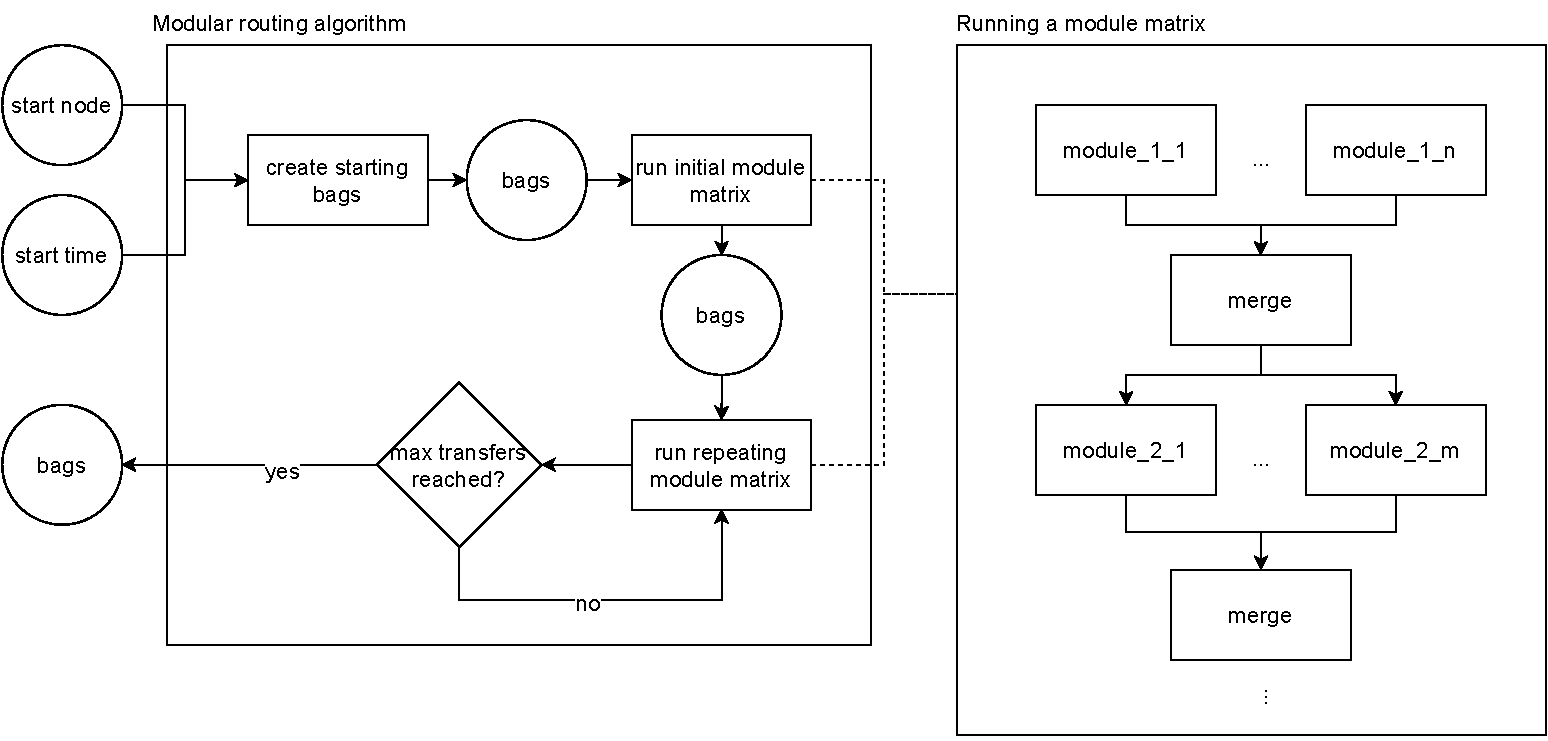
\includegraphics[scale=0.40]{Figures/method/modular_routing_algorithm}
    \caption{Modular Routing Algorithm}
    \label{fig:modular_routing_algorithm}
\end{figure}


\subsubsection{Modules}
\label{subsubsec:modules}

In our experiments, we categorize four modules into two types: unscheduled and scheduled. 
The unscheduled modules consist of walking, free-floating vehicle sharing, and personal vehicle use and are based on MLC, while the scheduled module is public transport, which is based on McRAPTOR.

Walking is the simplest unscheduled module, it simply consists of running MLC on the walking graph.
The edges of the walking graph should contain the time it takes to traverse them by foot and should not have any monetary cost associated with them.

The free-floating vehicle sharing module is a bit more complex.
Before running MLC on the respective vehicle graph, the module filters our all bags that are located at a node where no free-floating vehicle is available.
In addition, the vehicle graph is augmented with a walking graph. 
This means that at nodes in the vehicle graph, where it is allowed to park the vehicle, there is an edge to the closest node in the walking graph.
This augmentation is necessary, as the output bags of the free-floating vehicle sharing module need to be associated with nodes in the walking graph, as it is the common network.
The module may also define any form of monetary cost.

For the personal vehicle module, we assume that there is only one personal vehicle and that it is located at the starting node.
Therefore, the module filters out all bags that are not located at the starting node.
Obviously, this module is only useful for the first trip, or more precisely, the module should only be used in the first row of the initial module matrix.
After that MLC is run on the vehicle graph again augmented with the walking graph.
% TODO: monetary cost

In comparison to the unscheduled modules, the public transport module does not use MLC, but McRAPTOR.
As a first step the module filters out all bags that are associated with a node that is not near a stop in the public transport system.
Next, the module performs a single iteration of McRAPTOR, which represents a single trip within the public transport system.
Last, the resulting bags have to be associated with nodes in the walking network again.
To do so, the modules simply use the node that is closest to the coordinates of the public transport stop.
Just like the free-floating vehicle module, the public transport module may define any form of monetary cost.

\subsubsection{Merging}
\label{subsubsec:merging}

The merging of bags after running multiple modules in parallel is quite simply.
Each bag represents a set of Pareto optimal labels and each bag is associated with a node.
We therefore merge bag-wise.
We differentiate between two cases:
\begin{enumerate}
    \item There is only one bag associated with a node.
    \item There are multiple bags associated with the same node.
\end{enumerate}
In the first case, we simply put the bag into the output bags.
In the second case, we create a new bag that contains all labels of all bags associated with the node, which might break the Pareto optimality of the labels.
Therefore, to restore the Pareto optimality of the labels, we remove all labels that are dominated by another label.

\subsubsection{Enhanced MLC \& McRAPTOR}
\label{subsubsec:enhanced_mlc_and_mcraptor}

To address the multi-objective optimization involving both time and monetary cost, we introduce enhancements to MLC and McRAPTOR. 
The standard versions of MLC and McRAPTOR do not adequately capture dynamic pricing models, which is necessary to realistically represent monetary costs.

% \paragraph{Challenges in the Original Algorithms} 
The original MLC associates a fixed cost with an edge, which cannot represent variable pricing, such as a bike-sharing tariff that costs 1euro per 15-minute increment. 
Labels are only updated by adding the cost of a given edge to the label's values.
Similarly, McRAPTOR updates the labels at each stop during route traversal only based on the information of the current trip and stop. 
With this McRAPTOR is unable to represent a pricing scheme that varies with the number of stops, like the one used by the Cologne Transport Authority.
Our proposed modifications involve the use of 'hidden values' within the labels that are used by these algorithms. 
These hidden values carry additional information which is not considered when comparing labels, but that may be used to update cost dynamically.

In the case of MLC, the hidden values may be updated along any edge, just like the regular values of the label.
A hidden value, may carry information on how long the current trip with the shared vehicle is.
We then additionally allow defining a function that updates while traversing an edge and may use the values and hidden values both before and after the traversal to do the update.
With this functionality it is easy to increment the cost by 1euro every time the time spent on the trip exceeds the 15-minute interval.

Similarly, the hidden values may be updated during McRAPTOR after every iteration of a stop.
We can, therefore, store how many stops the current trip already traversed and if that number exceeds four, we can easily increase the price from 2.20euro to 3.20euro.

Additionally, as the concept of hidden values isn't specific to MLC or McRAPTOR, the hidden values can be transferred across iterations and modules.
To understand the benefit, again consider the example of the pricing of the Cologne Transport Authority.
The ticket that costs 3.20euro allows traveling any number of trips within Cologne, no matter if it is necessary to change to a different trip.
Therefore, if we were to first travel two stations with one trip and then get out to catch another trip that consists of five stops, we would still have the information that we already commuted two stops.
Therefore, we can charge 3.20euro, instead of charging 2.20euro two times, which is more realistic.
These enhanced versions of MLC and McRAPTOR are used in our modules, so that we can use the more realistic dynamic pricing schemes.

While running our experiment, we see that MLC based modules present a significant computational bottleneck.
We observe that in order to calculate our metric, we don't actually need to have the labels of every single node, but only of those, that impact the X-minute city and time Pareto front.
We therefore introduce a runtime optimization into MLC, which eliminates some bags from being processed that are guaranteed to not impact the Pareto front.
While iterating the unprocessed bags in MLC, we keep track of the minimum time required to reach a POI node of each category for each cost value.
If we encounter a bag whose time and cost values are both greater than the minimum time and cost values for all categories, we can safely discard this bag, as it will not impact the Pareto front.


\subsubsection{Example}
\label{subsubsec:example}

To illustrate our algorithm, we will now go through an example step by step.
The module configuration we use in our example represents travelling by free-floating vehicle sharing, public transport and walking.
The initial module matrix just contains the walking module, in order to initially reach the free-floating vehicles, as well as, the public transport stops.
The repeating module matrix consists of first the free-floating vehicle sharing module and the public transport module in parallel and then the walking module.
It can be seen in Figure \ref{fig:example_module_matrix}.


\begin{figure}[ht]
\centering
\[
\begin{pmatrix}
\text{free-floating vehicle} & \text{public transport} \\
\text{sharing module} & \text{module} \\
\\
\text{walking} & \\
\end{pmatrix}
\]
\caption{Example Repeating Module Matrix}
\label{fig:example_module_matrix}
\end{figure}

In our example, we assume that both public transport and vehicle sharing has some form of cost associated with it.
The objective is to minimize arrival time and cost.
We also only consider a maximum of two trips.

First we run the initial modules, which in our case is just the walking module on the starting bags.
As the starting bags only consist of one non-empty bag at the starting node with exactly one label, running MLC on the walking graph is equivalent to running Dijkstra's algorithm.
In the real-world this represents walking to all nodes in the walking network from the start node.
Note, that after the initial walking module all bags only contain exactly one label, as the cost to go anywhere by foot is zero.

Next the modules of the first row of the repeating matrix are run.
In the real-world this means that after an initial walk the traveler would either drive with a free-floating vehicle starting from a location where one is available or commute by public transport starting from one stop.
For public transport one could imagine that we commute with all possible trips from all stops and update the bags of the stops along each route accordingly.
After running these modules and merging their result bags, each bag may contain more than one label, as public transport and driving with a vehicle may be faster than walking, but also cost money.
It may even be that some bags contain three different labels, if, for example, driving with a vehicle is the fastest but also costs the most money and commuting by public transport is faster than walking.
The next step consists of running the second row of the repeating module matrix, which in our case is the walking module again.
Running the walking module in the repeating module matrix is important in order to reach nearby POIs after commuting through the public transport system.
After that the repeating module matrix is run again, as we consider a maximum of two trips.
The result of the second run of the repeating module matrix is our final result.



\subsection{Integrated Accessibility Analysis Routine}
\label{subsec:combining}

We embed the routing algorithm described in Section \ref{subsec:routing_algorithms} in our accessibility analysis routine to compute the metric described in Section \ref{subsec:metric}.
Our accessibility analysis routine consists of three parts: the input routine, the main routine and the metrics routine.

% Input routine
\begin{figure}
    \centering
    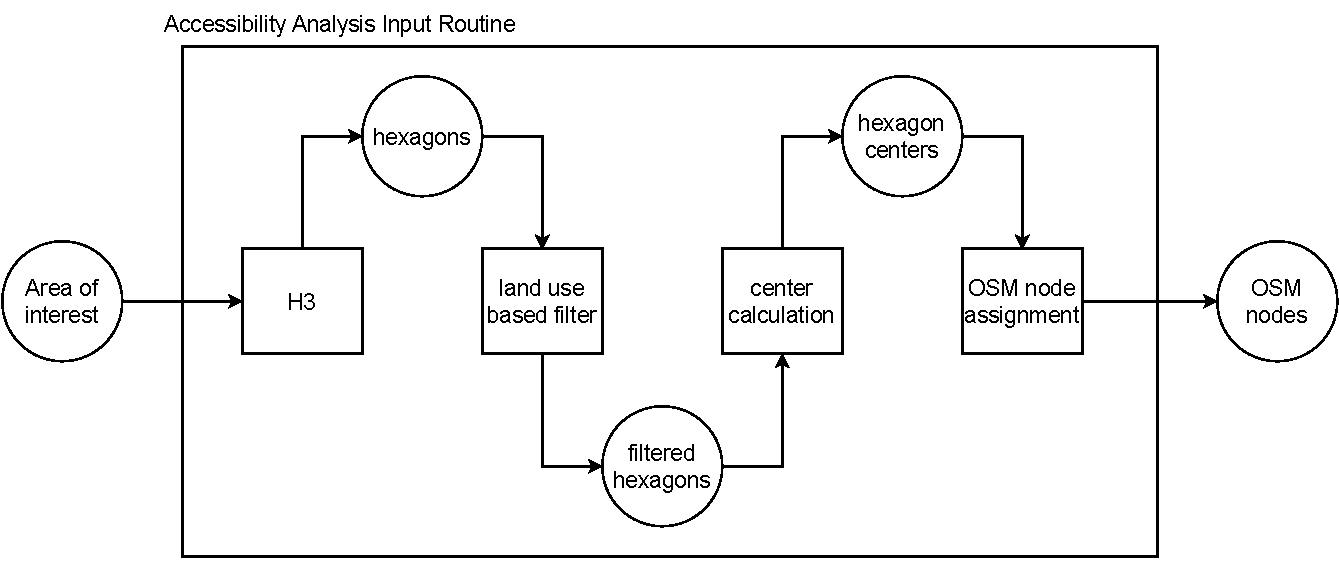
\includegraphics[scale=0.60]{Figures/method/input_routine}
    \caption{Input Routine}
    \label{fig:input_routine}
\end{figure}
In the input routine, depicted in Figure \ref{fig:input_routine}, we first create an even grid that covers the whole area of interest, for example a city.
To create such a grid, we use H3 \shortcite{H3H3}, which uses hexagons to evenly discretize an area.
Our goal will be to calculate our metric for each hexagon, so that we get detailed spatial information about the accessibility in the area of interest.
The chosen H3 resolution determines the size of these hexagons: a higher resolution means smaller hexagons, enhancing the granularity of our analysis. 
As such, selecting an appropriate H3 resolution is pivotal as it allows us to calculate our metrics for each hexagon with increased spatial accuracy, yielding a detailed spatial dataset that reflects the accessibility variations within the area of interest.
We recommend a resolution of nine, which corresponds to a hexagon edge length of roughly 200 meters, as it is a good compromise between accuracy and computation time.
The input routine also filters out uninteresting hexagons.
For, example we filter out hexagons that don't contain any residential areas, as there are no people living there is no need to access any amenities.
Next the input routine retrieves the centroid of each hexagon and then calculates the Euclidean distance between the centroids and the OSM nodes in order to assign the closest OSM node to each centroid.
The result of the input routine is a set of OSM nodes, for which we want to compute the accessibility.

% TODO:
% START this does not belong here
% The underlying street network needs to be larger than the area of interest.
% Otherwise, border regions will have a lower accessibility than they should, as the street network is incomplete.
% END this does not belong here


% Main routine
\begin{figure}
    \centering
    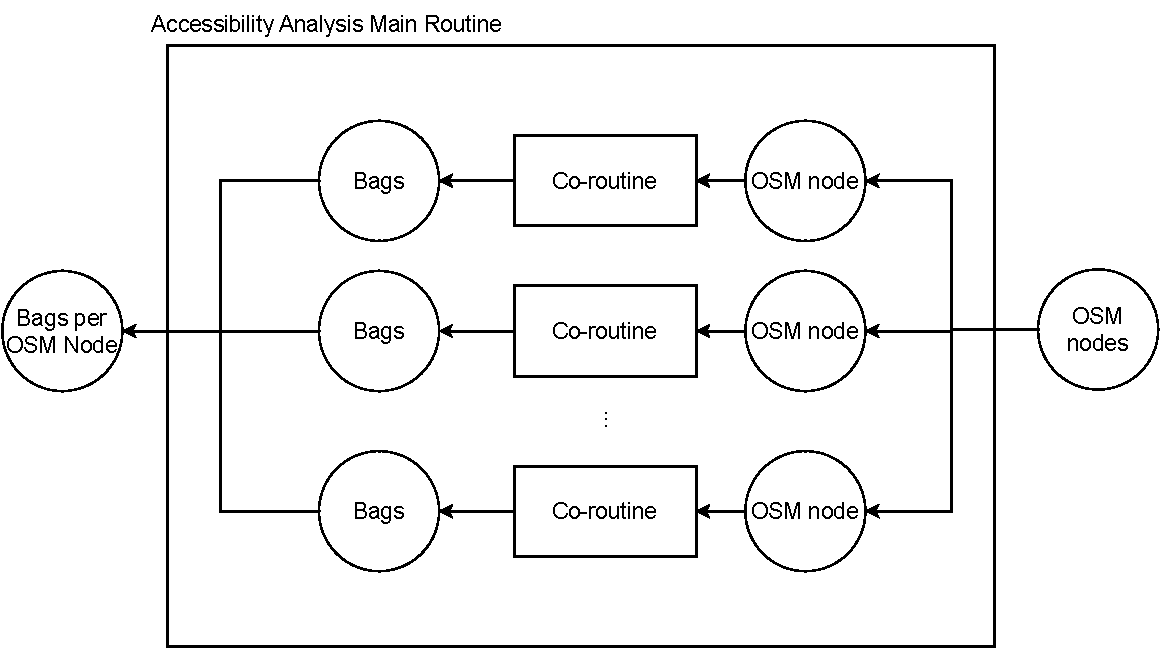
\includegraphics[scale=0.75]{Figures/method/main_routine}
    \caption{Main Routine}
    \label{fig:main_routine}
\end{figure}
The main routine, depicted in Figure \ref{fig:main_routine}, calls our scaffolding routing algorithm described in Section \ref{subsec:routing_algorithms} on each OSM node provided by the input routine.
This results in a set of Bags for each node.

% Metrics routine
\begin{figure}
    \centering
    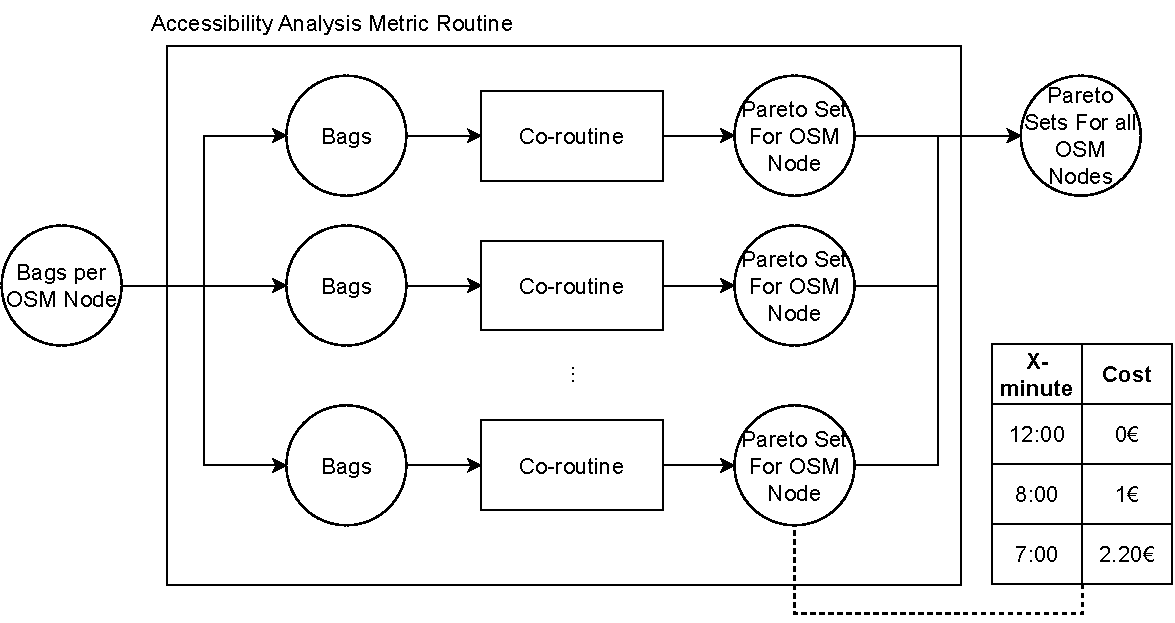
\includegraphics[scale=0.75]{Figures/method/metric_routine}
    \caption{Metric Routine}
    \label{fig:metric_routine}
\end{figure}
The metrics routine, depicted in Figure \ref{fig:metric_routine}, processes the bags into Pareto sets, where one entry in the Pareto set is a tuple of the X-minute city metric and the related cost.
To do so, we process each collection of bags separately - one co-routine for each OSM node/collection of bags.

\begin{figure}
    \centering
    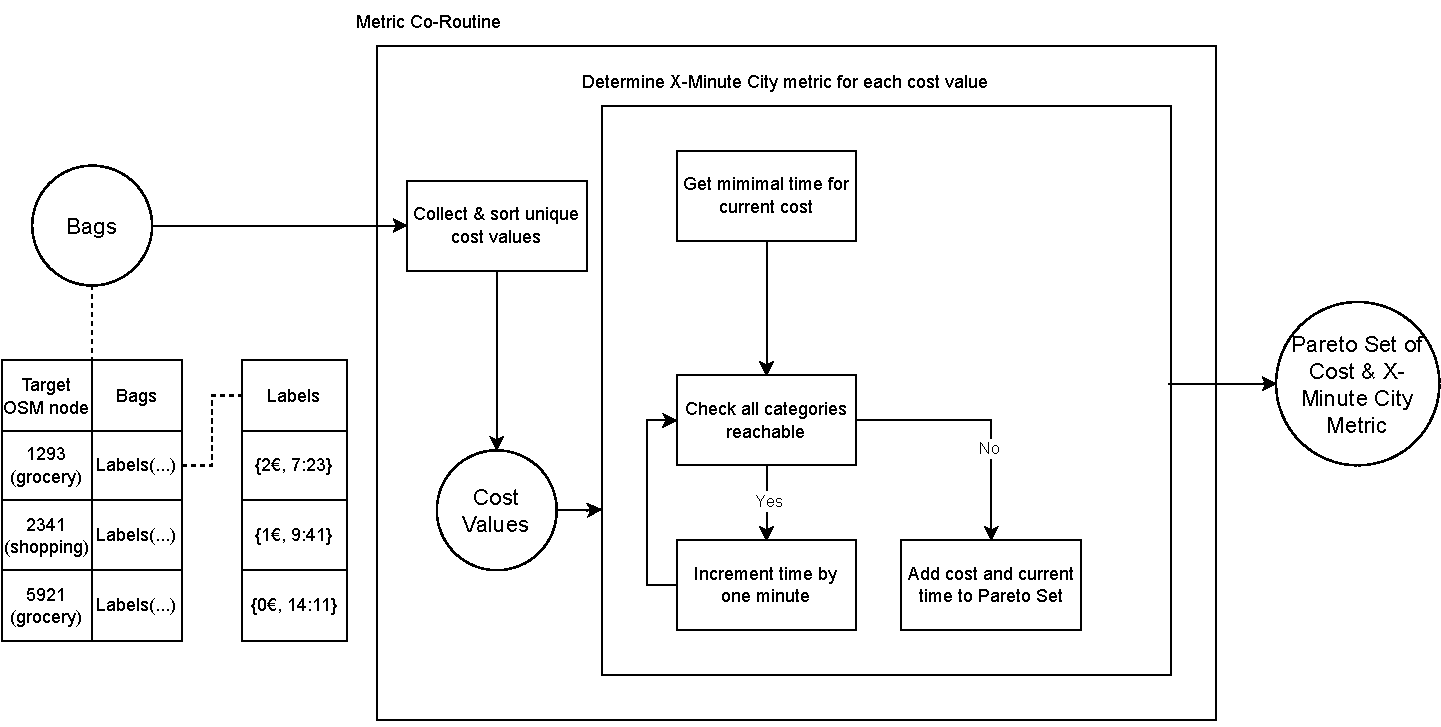
\includegraphics[scale=0.50]{Figures/method/metric_coroutine}
    \caption{Metric Co-Routine}
    \label{fig:metric_co_routine}
\end{figure}
The co-routine is depicted in Figure \ref{fig:metric_co_routine} and works as follows.
We start by collecting all unique cost values in each label in each bag and then sort them in ascending order.
For each cost value we then determine the associated X-minute city metric.
We do so by checking whether every category is reachable given the cost value and an iteratively increasing time value.
We start with a time value that is equal to the minimum time across all labels.
If all categories are reachable, we've found the X-minute city metric, which together with the cost value is added to the Pareto set.
If not, we increase the time value by one minute and check again.
We repeat this until all cost values are processed.
The result is a Pareto set for each OSM node/collection of bags.

\clearpage
\section{Experiment}
\label{sec:experiment}

We apply our method to the city of Cologne, to retrieve insights about how different modes of transport interact and how they contribute to the accessibility of the city.
As we want to compare different modes of transport, we will calculate the metric multiple times for different scenarios, each with a different combination of modes of transport.

\subsection{Scenarios}
\label{subs:scenarios}

No matter, the mode of transport, we always allow for walking, for two reasons.
First, walking is the most accessible mode of transport, available to almost everyone and without any additional costs.
Second, most other modes of transport require walking at some point, be it to the next bus stop or to the next available bicycle.

The first scenario we consider is our baseline scenario, which only considers walking.
This scenario measures what is possible without any additional infrastructure. 
Distinct from other scenarios, it does not require any additional cost, thus presenting the most basic form of urban mobility.

Building on this, the second scenario we consider is the scenario of only walking. 
We consider this scenario as the benchmark scenario, as we hope to achieve similar (or even better) results with more sustainable modes of transport.
Therefore, we use it to answer the question of how competitive sustainable modes of transport are in comparison to the traditional mode of travel by car. 

Transitioning from the simplest form of mobility, the third scenario, focused on public transport, becomes essential to understand the effectiveness and accessibility of urban transit systems. 
This scenario evaluates how well-connected and time-efficient public transportation networks are, and their role in reducing reliance on personal vehicles. 
It also investigates the impact of public transport on urban mobility and its potential in contributing to a more sustainable urban environment. 
Specifically, it assesses whether public transport is a viable alternative to the personal car and whether it actually offers significant advantages over walking, considering the X-minute city metric.

Next, in the fourth scenario, we shift our focus to the dynamics of bicycle sharing systems. 
This scenario is important for assessing the feasibility and attractiveness of cycling as a primary mode of transportation in urban areas. 
We will directly compare it to the public transport scenario, to understand which sustainable mode of transport is superior.

Finally, the fifth scenario combines public transport and bicycle sharing, offering insights into the synergy between these two modes of transport.
For the sake of brevity, we refer to this scenario as the combined scenario.
This integrated approach mirrors a growing trend in urban mobility solutions, where multi-modal transport options are increasingly favored. 
It underscores how this combination can bridge the gaps in accessibility and efficiency found when each mode is used independently. 
This scenario is expected to be the most competitive against cars, offering a comprehensive and sustainable urban transit model that could reshape the landscape of city mobility.

We summarize the scenarios in Table \ref{table:scenarios}.

\begin{table}[h]
\centering
\begin{tabular}{|p{4cm}|p{5cm}|p{4cm}|}
\hline
\textbf{Scenario} & \textbf{Modules} & \textbf{Key Points} \\
\hline
Walking & Walking & Baseline scenario \\
\hline
Personal Car & Personal Vehicle, Walking & Benchmark scenario \\
\hline
Public Transport & Public Transport, Walking & Evaluate the effectiveness public transport systems \\
\hline
Bicycle Sharing & Vehicle Sharing, Walking & Evaluate the effectiveness of bicycle sharing systems \\
\hline
Combined & Public Transport, Bicycle Sharing, Walking & Evaluate the effectiveness of sustainable multi-modal transport systems \\
\hline
\end{tabular}
\caption{Scenarios for Urban Mobility Analysis}
\label{table:scenarios}
\end{table}

The specific configuration of the module matrices for each scenario can be found in Appendix \ref{app:experiment_module_matrix_configuration}.

\subsection{Data}
\label{subs:data}

To calculate the Pareto sets of the X-minute city metric for the different scenarios, we use four different datasets.
First, we require data that depicts the street network of the city of Cologne.
Second, we need to know the locations of the POIs, which we want to reach.
Third, we need to know the locations of the public transport stops, as well as, the schedules of the public transport.
For the bicycle sharing scenario, we also need to know the locations of the bicycles.
Lastly, we also use land use data to identify where residential areas are located, so that we can calculate the X-minute city metric only for these areas.

As we will query spatial datasets of various formats, from different sources, the area covered by the datasets will not be the same.
Therefore, we first define an area of interest and later trim the datasets to this area.
In our case, this area is defined as the area of the administrative district of Cologne, specifically the "Stadtkreis Köln".
We retrieve the specific boundary of this area with the help of the Overpass API \shortcite{OverpassAPIOverpass}.
The specific query can be found in Appendix \ref{app:overpass_query} and the resulting region can be seen in Figure \ref{fig:area_plus_buffer}.

\begin{figure}
  \begin{center}
    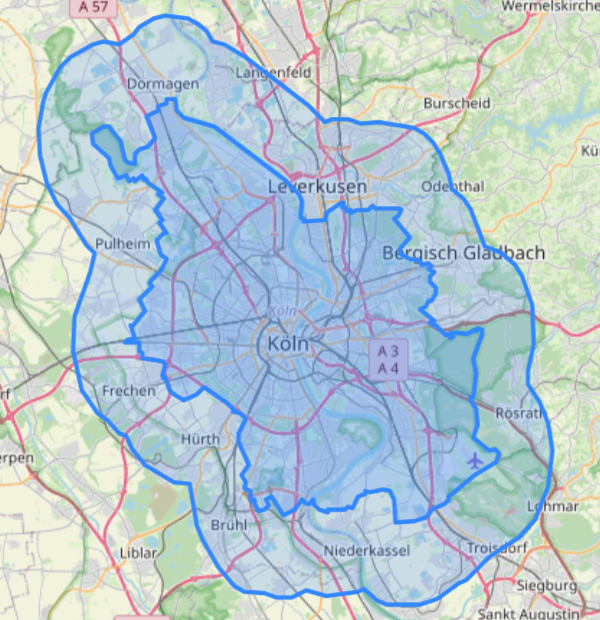
\includegraphics[width=0.55\textwidth]{Figures/experiment/area_plus_buffer.png}
  \end{center}
  \caption{Area of Interest and Buffer Region}\label{fig:area_plus_buffer}
\end{figure}

Additionally, the Figure also shows a buffer region around our area of interest.
This larger region adds a buffer of approximately 5 km and is used by some in parts of our data processing.


\subsubsection{Street Network \& POIs}
\label{subs:street_network_pois}

For the street network and the POIs, we use data from OpenStreetMap (OSM) \shortcite{OpenStreetMap}.
To use OSM data in practice various tools and services have been developed.
Among these we use, pyrosm \shortcite{Pyrosm} which is a Python library designed specifically for reading OSM data in different formats and conducting data processing operations.
Through pyrosm, we can automatically fetch data from sources like Geofabrik \shortcite{GeofabrikDownloadServer} and BBBike \cite{BBBikeExtractsOpenStreetMap}, which are two of the most popular OSM data providers.
In our case, we use the data for the city of Cologne from BBBike.
However, due to the flexibility of pyrosm, it is easily possible to use data from other sources as well and expand our analysis to other cities.

After retrieving the data, we retrieve a graph representation of the street network trimmed to the buffered area of interest.
Using the buffered region is important, because without it calculating the X-minute city metric at the border of the area of interest would result in a higher value than the actual value.
As a last cleaning step, we remove all nodes, that are not part of the largest weakly connected component.
A weakly connected component is a subgraph in which, if all directed edges were treated as undirected, any two vertices from the subgraph would be connected.
Multiple weakly connected components in graphs derived from OSM data, mostly happen at the border of the considered area and can be neglected.

Because we consider multiple different modes of transport on the network, it is important to filter out all edges that are not accessible by the respective mode of transport.
To do so, we use pyrosm's built-in filtering functionality.
For reproducibility, we list the filters that pyrosm uses in Appendix \ref{app:pyrosm_network_filter}.

To retrieve the POIs, we use the Overpass API \shortcite{OverpassAPIOverpass}.
We retrieve all POIs that fall into one of our predefined categories specified in Section \ref{subsec:metric} inside the area of interest plus the buffer mentioned before.

\subsubsection{Public Transport}
\label{subs:public_transport}

To handle public transport data, we use the General Transit Feed Specification (GTFS) \shortcite{GTFS}.
To retrieve it we rely on the Mobility Database \shortcite{MobilityDatabase}.
This database serves as an open-source repository containing links to publicly available GTFS feeds globally, standing as the subsequent version of TransitFeeds \shortcite{OpenMobilityDataPublicTransit}.
Similarly to the OSM data, we trim the GTFS data to the area of interest plus the buffer.
The GTFS data is also cleaned and converted into a format that is more suitable for our algorithm, or more specifically McRAPTOR, which is part of our algorithm.
Specifically, there are two major incompatibilities between the GTFS specification and RAPTOR's notion of routes and trips.
Firstly, each trip belonging to a single route in RAPTOR visits the same stops in the same order.
It is not possible that a trip skips some stops that another trip of the same route visits, much less use a completely different sequence of routes.
In GTFS routes do allow that, as they are much more a group of trips that is presented to the rider under the same name or identifier.
Secondly, GTFS trips allow visiting the same stop multiple times, which is not allowed in RAPTOR.
To overcome these difference we split up routes into smaller routes, that follow the same sequence of stops.
Additionally, e also remove circular trips, altogether.


\subsubsection{Bicycle Sharing}
\label{subs:bicycle_sharing}

Our bicycle sharing data was retrieved from the NextBike API over a time period of one year.
The data consists of all trips that were made with the NextBike system in the city of Cologne from the 15th of January 2022 to the 31st of August 2023.
To get representative samples of the locations of all bicycles we employ the following strategy.
We first discretize the data spatially and temporally.
For the temporal discretization, we derive the location of each bicycle every hour.
For the spatial discretization, we use H3 hexagons with a resolution of 9.
The resulting data is the information how many bicycles were at each hexagon at each hour.
This data is then used as an input for k-medoids clustering \shortcite{rdusseeun1987clustering} with a k of 4.
K-medoids, also known as PAM (Partitioning Around Medoids) algorithm, is a clustering technique that partitions a dataset into K clusters, where each is assigned a medoid, that is the most centrally located object in a cluster. 
Unlike K-means, which uses mean values as cluster centers, K-medoids an actual data point as the center of a cluster.
This has the advantage that the centers are part of the dataset and therefore are realistic samples.
We use the resulting medoids as different configurations of the locations of the bicycles.

\subsubsection{Land Use}
\label{subs:land_use}

To identify the residential areas, we use the land use data from the CORINE Land Cover (CLC) project \shortcite{CORINELandCover}.
The data covers the whole of Europe and is publicly available, which again makes it possible to expand our analysis to other cities in Europe.
We trimmed the data to the area of interest and then filtered for the land use types "Continuous Urban Fabric" and "Discontinuous Urban Fabric".
These two land use types represent the residential areas of the city.
The residential areas inside the area of interest are shown in Figure \ref{fig:input_hexagons_residential_areas}.
Additionally, the Figure shows the hexagons of resolution 9 that are found inside the residential areas.

\begin{figure}
  \begin{center}
    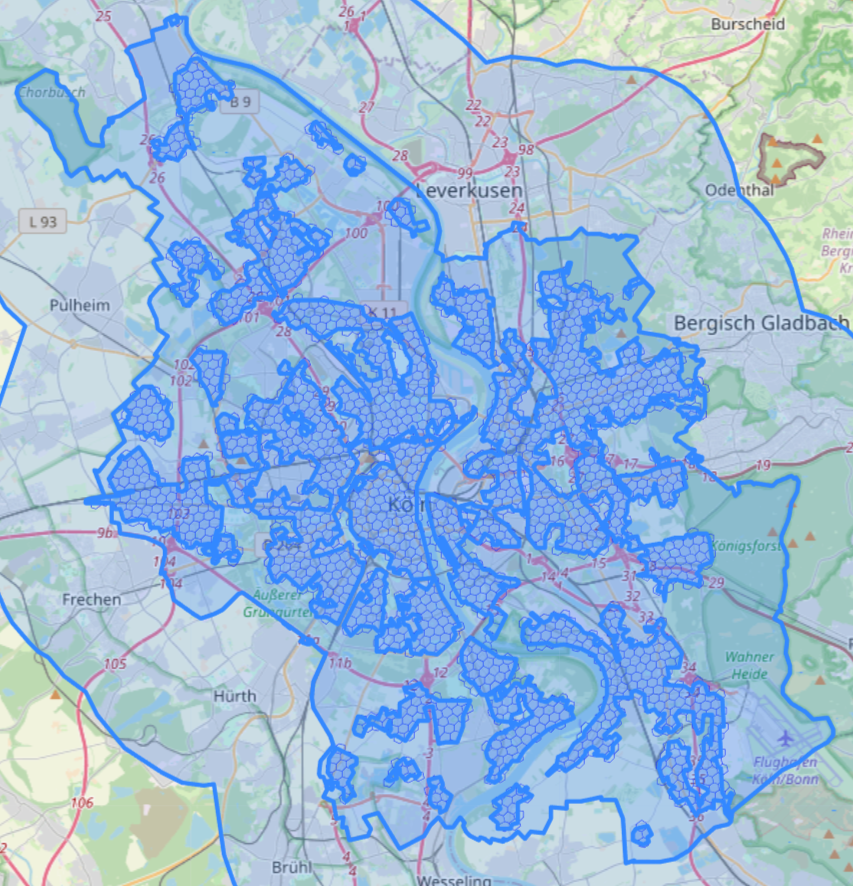
\includegraphics[width=0.65\textwidth]{Figures/experiment/input_hexagons_residential_areas.png}
  \end{center}
  \caption{Area of Interest and Buffer Region with Residential Areas and Input Hexagons}
  \label{fig:input_hexagons_residential_areas}
\end{figure}


\subsection{Assumptions}
\label{subs:assumptions}

To calculate the X-minute city metric we have to abstract from reality to some degree.
We do so by making the following plausible assumptions.

Firstly, we assume that travelling along an edge on the street network, by walking, cycling or driving, is always proportional to the length of the edge.
To obtain the time it takes to travel along an edge, we divide the length of the edge by the speed of the mode of transport.
The different speeds for the different modes of transport are listed in Table \ref{table:speeds}.

\begin{table}[h]
\centering
\begin{tabular}{|c|l|}
\hline
\textbf{Mode} & \textbf{Speed (m/s)} \\
\hline
Walking & 1.4 \\
\hline
Cycling & 4.0 \\
\hline
Driving & 11.0 \\
\hline
\end{tabular}
\caption{Speeds for Different Modes of Transport}
\label{table:speeds}
\end{table}

The walking speed is consistent with the measurement that \shortciteA{willberg15minuteCityAll2023} made in their study.

We also pose some assumption on the transitioning between different modes of transport, as well as, in the case of public transport, the transfer time at the stops.
For the transfer time at stops we assume a fixed time of one minute.
To transition from any OSM network-based mode of transport to public transport, we assume that the stop is precisely at the location the closest node of the OSM network.
As OSM networks contain public transport stops, there should be no difference between the two.
Similarly, we assume that the bicycles are located at the closest node of the OSM network.
As the OSM network, especially in city is very dense, this assumption is reasonable.
We also assume that bicycles and cars can be parked anywhere on their respective network for the sake of simplicity.


\subsubsection{Pricing}
\label{subs:pricing}

We try to implement a pricing scheme in our scenarios that represents the real-world circumstances as closely as possible.

For bicycle sharing, we use the pricing scheme of NextBike, which is 1euro every 15 minutes.
To depict this we add a hidden value to the labels processed in MLC that depicts how long the current bicycle trip is.
As two consecutive bicycle trips are considered separately we nullify this hidden value after each run of MLC.

For public transport, we use the pricing scheme of the Cologne Transport Authority (KVB), which is 2.20euro for trips that span four stops or less.
For any trip that spans more than four stops or any multitude of trips the KVB charges 3.20euro.
To depict this we add a hidden values to the labels processed in McRAPTOR that depicts how many stops the traveler already traversed.
Because two consecutive trips are considered together, we don't need to nullify the hidden value.

% TODO: personal car



%%%%%%%%%%%%%%%%%%%%%%%%%%%%%%%%%%%%%%%%%%%%%%%%%%%%%%%%%%%%%
%APPENDICES
%%%%%%%%%%%%%%%%%%%%%%%%%%%%%%%%%%%%%%%%%%%%%%%%%%%%%%%%%%%%%


\appendix
\renewcommand*{\thesection}{\Alph{section}}\textbf{}

% APPENDIX A
\clearpage
\section{Appendix - Overpass Query for Boundary of Cologne}
\label{app:overpass_query}
\begin{verbatim}
[out:json][timeout:50];
area["name"="Köln"]->.searchArea;
relation["boundary"="administrative"]["admin_level"="6"](area.searchArea);
out body;
>;
out skel qt;
\end{verbatim}

\section{Appendix - Pyrosm Network Filter}
\label{app:pyrosm_network_filter}

Pyrosm filters out all ways that have the following tags:

\begin{table}[h]
\centering
\caption{Driving Filter}
\begin{tabular}{|c|p{10cm}|}
\hline
\textbf{Key}         & \textbf{Values}                                                                                                             \\ \hline
area                 & yes                                                                                                                         \\ \hline
highway              & cycleway, footway, path, pedestrian, steps, track, corridor, elevator, escalator, proposed, construction, bridleway, abandoned, platform, raceway \\ \hline
motor\_vehicle       & no                                                                                                                          \\ \hline
motorcar             & no                                                                                                                          \\ \hline
service              & parking, parking\_aisle, private, emergency\_access                                                                         \\ \hline
\end{tabular}
\end{table}


\begin{table}[h]
\centering
\caption{Walking Filter}
\begin{tabular}{|c|p{10cm}|}
\hline
\textbf{Key}         & \textbf{Values}                                                                                                             \\ \hline
area                 & yes                                                                                                                         \\ \hline
highway              & cycleway, motor, proposed, construction, abandoned, platform, raceway, motorway, motorway\_link                             \\ \hline
foot                 & no                                                                                                                          \\ \hline
service              & private                                                                                                                     \\ \hline
\end{tabular}
\end{table}


\begin{table}[h]
\centering
\caption{Cycling Filter}
\begin{tabular}{|c|p{10cm}|}
\hline
\textbf{Key}         & \textbf{Values}                                                                                                             \\ \hline
area                 & yes                                                                                                                         \\ \hline
highway              & footway, steps, corridor, elevator, escalator, motor, proposed, construction, abandoned, platform, raceway, motorway, motorway\_link \\ \hline
bicycle              & no                                                                                                                          \\ \hline
service              & private                                                                                                                     \\ \hline
\end{tabular}
\end{table}


\section{Appendix - Categories and Their Corresponding OSM Tags}
\label{app:categories_and_osm_tags}

\begin{table}[ht]
\centering
\caption{Categories and Their Corresponding OSM Tags}
\label{tab:categories}
\footnotesize
\begin{tabular}{|l|l|p{10cm}|}
\hline
\textbf{Category} & \textbf{OSM Key} & \textbf{OSM Value} \\ \hline
Grocery           & shop             & alcohol, bakery, beverages, brewing supplies, butcher, cheese, chocolate, coffee, confectionery, convenience, deli, dairy, farm, frozen food, greengrocer, health food, ice-cream, pasta, pastry, seafood, spices, tea, water, supermarket, department store, general, kiosk, mall \\ \hline
Education         & amenity          & college, driving school, kindergarten, language school, music school, school, university \\ \hline
Health            & amenity          & clinic, dentist, doctors, hospital, nursing home, pharmacy, social facility \\ \hline
Banks             & amenity          & atm, bank, bureau de change, post office \\ \hline
Parks             & leisure          & park, dog park \\ \hline
Sustenance        & amenity          & restaurant, pub, bar, cafe, fast-food, food court, ice-cream, biergarten \\ \hline
Shops             & shop             & department store, general, kiosk, mall, wholesale, baby goods, bag, boutique, clothes, fabric, fashion accessories, jewelry, leather, watches, wool, charity, secondhand, variety store, beauty, chemist, cosmetics, erotic, hairdresser, hairdresser supply, hearing aids, herbalist, massage, medical supply, nutrition supplements, optician, perfumery, tattoo, agrarian, appliance, bathroom furnishing, do-it-yourself, electrical, energy, fireplace, florist, garden centre, garden furniture, fuel, glaziery, groundskeeping, hardware, houseware, locksmith, paint, security, trade, antiques, bed, candles, carpet, curtain, flooring, furniture, household linen, interior decoration, kitchen, lighting, tiles, window blind, computer, electronics, hifi, mobile phone, radio-technics, vacuum cleaner, bicycle, boat, car, car repair, car parts, caravan, fishing, golf, hunting, jet ski, military surplus, motorcycle, outdoor, scuba diving, ski, snowmobile, swimming pool, trailer, tyres, art, collector, craft, frame, games, model, music, musical instrument, photo, camera, trophy, video, videogames, anime, books, gift, lottery, newsagent, stationery, ticket, bookmaker, cannabis, copy shop, dry cleaning, e-cigarette, funeral directors, laundry, moneylender, party, pawnbroker, pet, pet grooming, pest control, pyrotechnics, religion, storage rental, tobacco, toys, travel agency, vacant, weapons, outpost \\ \hline
\end{tabular}
\normalsize
\end{table}

\section{Appendix - Experiment Module Matrix Configuration}
\label{app:experiment_module_matrix_configuration}

% walking step
    % initial_steps = [[walking_step]]
    % repeating_steps = []

\begin{figure}[ht]
    \centering
    \begin{subfigure}{0.45\linewidth}
        \centering
        \[
        \begin{pmatrix}
            \text{walking module} \\
        \end{pmatrix}
        \]
        \caption{Initial Matrix}
    \end{subfigure}
    \hfill
    \begin{subfigure}{0.45\linewidth}
        \centering
        \[
        \begin{pmatrix}
            \\
        \end{pmatrix}
        \]
        \caption{Repeating Matrix}
    \end{subfigure}
    \caption{Walking Scenario Module Matrices}
    \label{fig:walking_scenario_module_matrix}
\end{figure}

% combined mode 
    % initial_steps = [[walking_step]]
    % repeating_steps = [
    %     [bicycle_step, public_transport_step],
    %     [walking_step],
    % ]

\begin{figure}[ht]
    \centering
    \begin{subfigure}{0.45\linewidth}
        \centering
        \[
        \begin{pmatrix}
            \text{walking module} \\
        \end{pmatrix}
        \]
        \caption{Initial Matrix}
    \end{subfigure}
    \hfill
    \begin{subfigure}{0.45\linewidth}
        \centering
        \[
        \begin{pmatrix}
            \text{free-floating vehicle} & \text{public transport} \\
            \text{sharing module} & \text{module} \\
            \\
            \text{walking module} & \\
        \end{pmatrix}
        \]
        \caption{Repeating Matrix}
    \end{subfigure}
    \caption{Combined scenario module matrices}
    \label{fig:combined_scenario_module_matrix}
\end{figure}

% personal car
    % initial_steps = []
    % repeating_steps = [[car_step]]


\begin{figure}[ht]
    \centering
    \begin{subfigure}{0.45\linewidth}
        \centering
        \[
        \begin{pmatrix}
            \\
        \end{pmatrix}
        \]
        \caption{Initial Matrix}
    \end{subfigure}
    \hfill
    \begin{subfigure}{0.45\linewidth}
        \centering
        \[
        \begin{pmatrix}
            \text{personal car module}\\
        \end{pmatrix}
        \]
        \caption{Repeating Matrix}
    \end{subfigure}
    \caption{Personal Car Scenario Module Matrices}
    \label{fig:personal_car_scenario_module_matrix}
\end{figure}

% bicycle only
    % initial_steps = [[walking_step]]
    % repeating_steps = [
    %     [bicycle_step],
    %     [walking_step],
    % ]


\begin{figure}[ht]
    \centering
    \begin{subfigure}{0.45\linewidth}
        \centering
        \[
        \begin{pmatrix}
            \text{walking module} \\
        \end{pmatrix}
        \]
        \caption{Initial Matrix}
    \end{subfigure}
    \hfill
    \begin{subfigure}{0.45\linewidth}
        \centering
        \[
        \begin{pmatrix}
            \text{public transport module} \\
            \text{walking module} \\
        \end{pmatrix}
        \]
        \caption{Repeating Matrix}
    \end{subfigure}
    \caption{Public Transport Scenario Module Matrices}
    \label{fig:public_transport_scenario_module_matrix}
\end{figure}

% public transport only
    % initial_steps = [[walking_step]]
    % repeating_steps = [[public_transport_step], [walking_step]]

\begin{figure}[ht]
    \centering
    \begin{subfigure}{0.45\linewidth}
        \centering
        \[
        \begin{pmatrix}
            \text{walking module} \\
        \end{pmatrix}
        \]
        \caption{Initial Matrix}
    \end{subfigure}
    \hfill
    \begin{subfigure}{0.45\linewidth}
        \centering
        \[
        \begin{pmatrix}
            \text{free-floating vehicle sharing module} \\
            \text{walking module} \\
        \end{pmatrix}
        \]
        \caption{Repeating Matrix}
    \end{subfigure}
    \caption{Bicycle Scenario Module Matrices}
    \label{fig:bicycle_scenario_module_matrix}
\end{figure}


\section{Appendix - Monthly Visits per Category}
\label{app:monthly_visits_per_category}

\paragraph{Grocery}
3 times per week according to \shortciteA{nilssonWhoShopsGroceries2015}.
Resulting in approximately 12 times per month.

\paragraph{Education}
5 times per week, as we assume that students visit their school or university 5 times per week.

\paragraph{Health}
5.09 per year according to \shortciteA{eurostatHowOftenYou2019}.
Resulting in approximately 0.42 times per month.

\paragraph{Banks}
9 per month according to \shortciteA{optconnectATMStatistics}.

\paragraph{Parks}
29 per year according to \shortciteA{nationalrecreationandparkassociationNumberTimesAmericans2016}.
Resulting in approximately 2.42 times per month.

\paragraph{Sustenance}
6.12 per month according to \shortciteA{saprykinImpactSocialMedia2016}.

\paragraph{Shops}
4 per month according to \shortciteA{businessplusHowOftenPeople2019}.






%%%%%%%%%%%%%%%%%%%%%%%%%%%%%%%%%%%%%%%%%%%%%%%%%%%%%%%%%%%%%
%BIBLIOGRAPHY
%%%%%%%%%%%%%%%%%%%%%%%%%%%%%%%%%%%%%%%%%%%%%%%%%%%%%%%%%%%%%

\clearpage
\renewcommand*{\thesection}{}\textbf{}

\bibliographystyle{apacite}
\bibliography{Bibliography.bib}


\end{document}
